% \clearpage
\subsection{Persisting Data} % (fold)
\label{sub:persisting_data}

When a program is running it uses variables and dynamically allocated memory to store the data it requires. These values exist within the memory allocated to the program when it was started. When the program ends its allocated memory is released, and the values stored within the program are lost. If values must be \emph{remembered} between executions then this data must be stored outside of the program. To achieve this you can save data from the program into files that are stored on the computer's hard drive or solid state drive (SSD).

\begin{figure}[h]
   \centering
   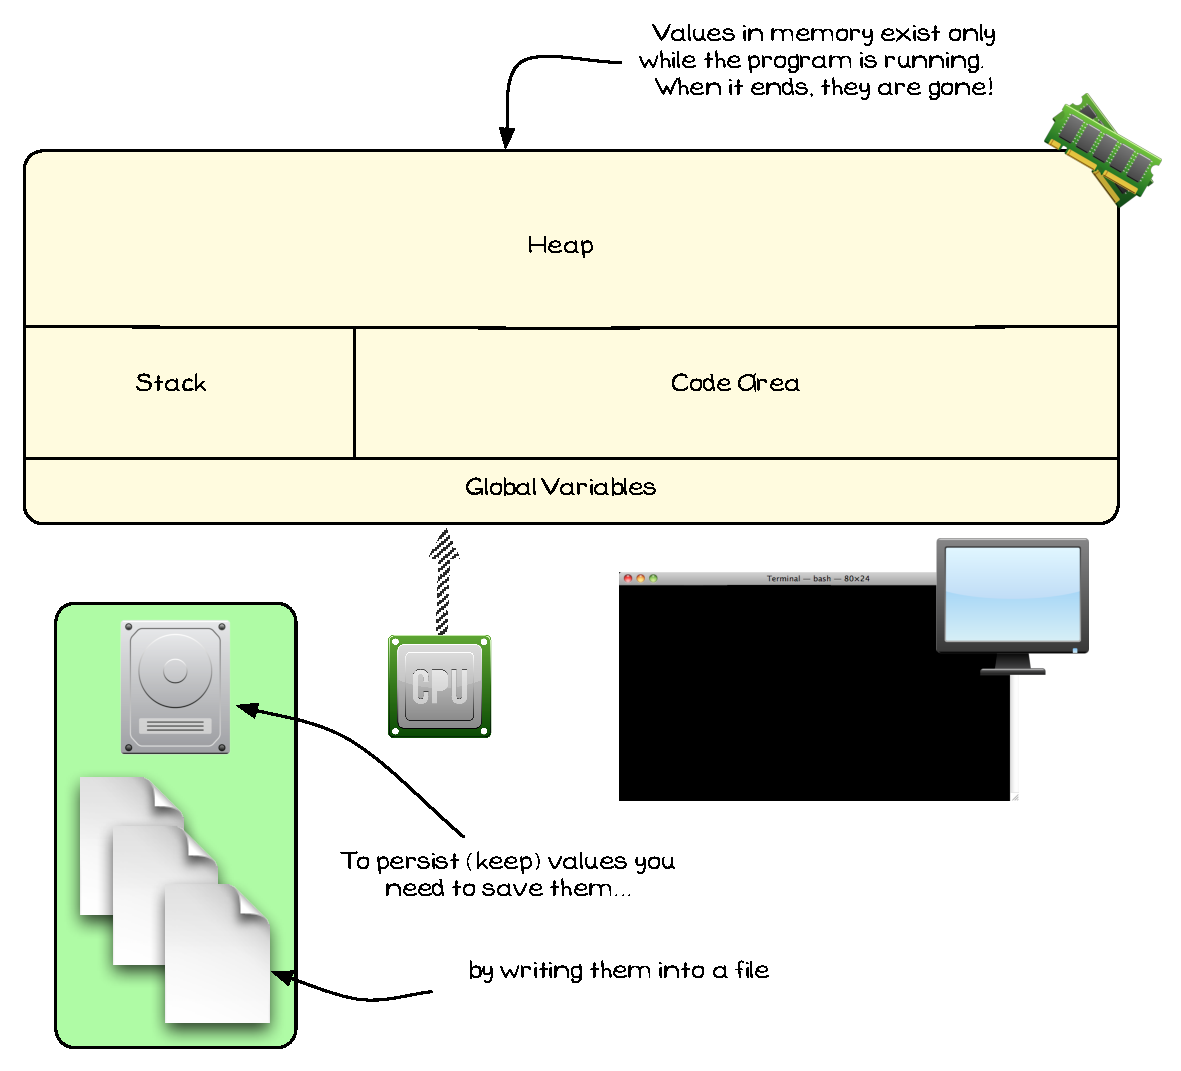
\includegraphics[width=\textwidth]{./topics/file-io/diagrams/PersistData} 
   \caption{When a program ends its data is gone, unless you save it to file}
   \label{fig:persist-data}
\end{figure}

\mynote{
\begin{itemize}
  \item Data stored within a program is lost when the program ends.
  \item To \emph{remember} data between executions it must be saved to file.
  \item The files are stored in a persistent way on a hard drive, or solid state drive.
  \item Hard drives, and solid state drives, are as data storage devices to persist data needed by programs on the computer.
\end{itemize}
}

% subsection persisting_data (end)